%%%%%%%%%%%%%%%%%%%%%%%%%%%%%%%%%%%%%%%%%%%%%%%%%%%%%%%%%%%%%%%%%%%%%%%%%%%%%%%%%%
\begin{frame}[fragile]\frametitle{}
\begin{center}
{\Large Introduction to AI Agents}
\end{center}
\end{frame}

%%%%%%%%%%%%%%%%%%%%%%%%%%%%%%%%%%%%%%%%%%%%%%%%%%%%%%%%%%%
\begin{frame}[fragile]\frametitle{What Even Is an AI Agent?}
No widely accepted definition exists, but here's a practical one:

\begin{columns}
    \begin{column}[T]{0.6\linewidth}
		\begin{itemize}
			\item \textbf{Generative AI:} Great at understanding and generating content
			\item \textbf{Agentic AI:} Goes further, understands, generates content, \textbf{and performs actions}
		\end{itemize}

    \end{column}
    \begin{column}[T]{0.4\linewidth}
        \begin{center}
        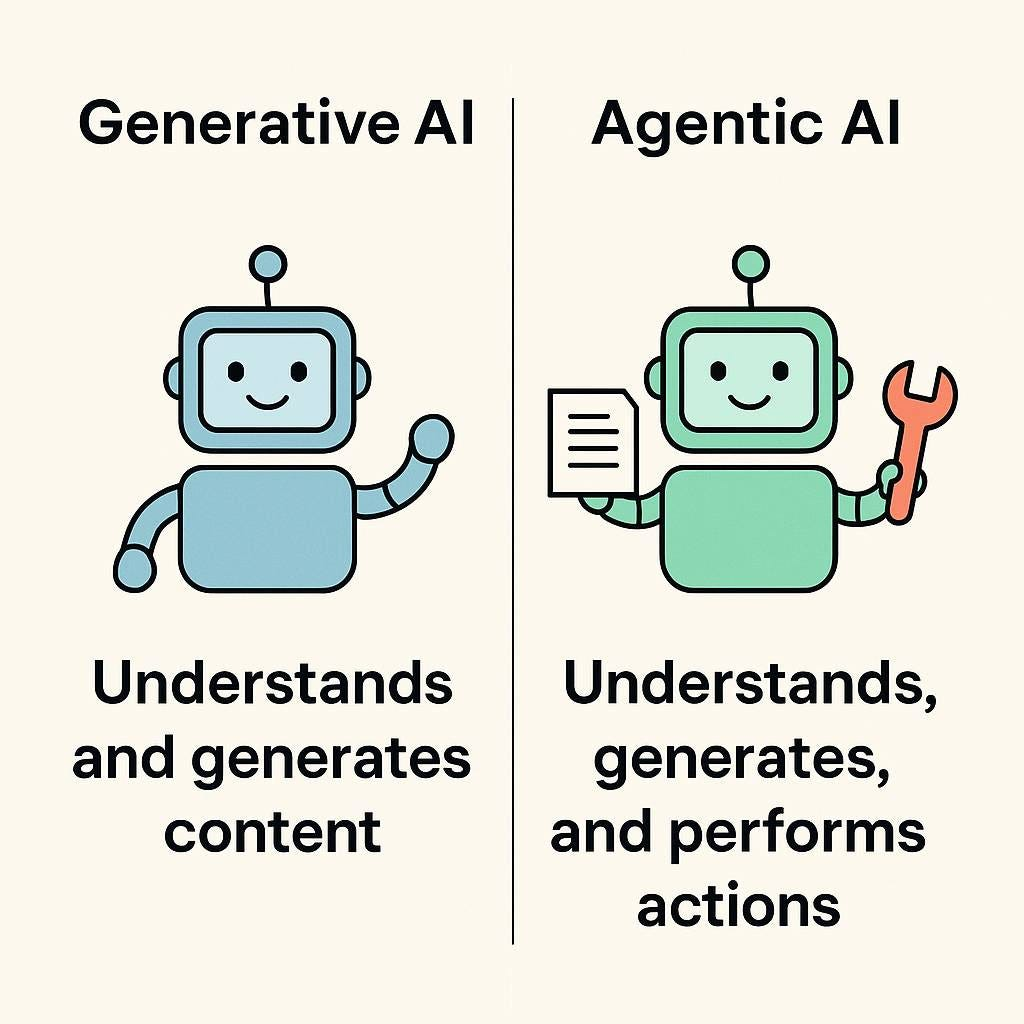
\includegraphics[width=\linewidth,keepaspectratio]{aiagents1}
		
		{\tiny (Ref: Agentic AI For Everyone - Aish \& Kiriti)}
        \end{center}
    \end{column}
  \end{columns}
  
The key differentiator is the ability to \textbf{take action}, not just respond  
\end{frame}

%%%%%%%%%%%%%%%%%%%%%%%%%%%%%%%%%%%%%%%%%%%%%%%%%%%%%%%%%%%%%%%%%%%%%%%%%%%%%%%%%%
\begin{frame}[fragile]\frametitle{The Evolution of AI Capabilities}
\begin{itemize}
    \item \textbf{Traditional Programming:} Needed code to operate
    \item \textbf{Traditional ML:} Needed feature engineering
    \item \textbf{Deep Learning:} Needed task-specific training
    \item \textbf{ChatGPT (2022):} Could reason across tasks without training
    \begin{itemize}
        \item Zero-shot learning (no examples needed)
        \item In-context learning (understands from instructions)
    \end{itemize}
    \item \textbf{Agents (2024):} Can actually \textbf{do things}, not just talk
\end{itemize}
\end{frame}

%%%%%%%%%%%%%%%%%%%%%%%%%%%%%%%%%%%%%%%%%%%%%%%%%%%%%%%%%%%%%%%%%%%%%%%%%%%%%%%%%%
\begin{frame}[fragile]\frametitle{Why Does "Taking Action" Matter?}
\begin{itemize}
    \item In 2022, ChatGPT was revolutionary because AI felt conversational
    \item By 2024, people wanted more than conversation, they wanted \textbf{execution}
    \item Examples of what users now expect:
    \begin{itemize}
        \item Instead of listing leads ? \textbf{email them directly}
        \item Instead of summarizing docs ? \textbf{file and create workflow tasks}
        \item Instead of suggesting products ? \textbf{customize landing pages}
    \end{itemize}
    \item This shift from \textbf{information} to \textbf{action} defines the agent era
\end{itemize}
\end{frame}

%%%%%%%%%%%%%%%%%%%%%%%%%%%%%%%%%%%%%%%%%%%%%%%%%%%%%%%%%%%%%%%%%%%%%%%%%%%%%%%%%%
\begin{frame}[fragile]\frametitle{How Do Agents Take Action?}
\begin{itemize}
    \item The magic lies in \textbf{tools} and \textbf{function calling}
    \item Agents are paired with APIs, plugins, or external systems
    \item Instead of just text responses, LLMs output structured commands:
    \begin{itemize}
        \item "Call the send\_email() function with these inputs..."
        \item "Fetch records from CRM using this query..."
        \item "Schedule a meeting for Tuesday at 2PM..."
    \end{itemize}
    \item \textbf{Mental model:} LLM = brain, Tools = hands
    \item Without tools, agents just talk. With tools, they act.
\end{itemize}
\end{frame}

%%%%%%%%%%%%%%%%%%%%%%%%%%%%%%%%%%%%%%%%%%%%%%%%%%%%%%%%%%%%%%%%%%%%%%%%%%%%%%%%%%
\begin{frame}[fragile]\frametitle{Future AI Applications}
\begin{itemize}
    \item What are future AI applications like?
    \begin{itemize}
        \item \textbf{Generative:} Generate content like text and images
        \item \textbf{Agentic:} Execute complex tasks on behalf of humans
    \end{itemize}
    \item How do we empower every developer to build them?
    \begin{itemize}
        \item \textbf{Co-Pilots:} Human-AI collaboration
        \item \textbf{Autonomous:} Independent task execution
    \end{itemize}
    \item 2024 is expected to be the year of AI agents
\end{itemize}
\end{frame}


%%%%%%%%%%%%%%%%%%%%%%%%%%%%%%%%%%%%%%%%%%%%%%%%%%%%%%%%%%%%%%%%%%%%%%%%%%%%%%%%%%
\begin{frame}[fragile]\frametitle{How AI Agent Works?}

	\begin{center}
	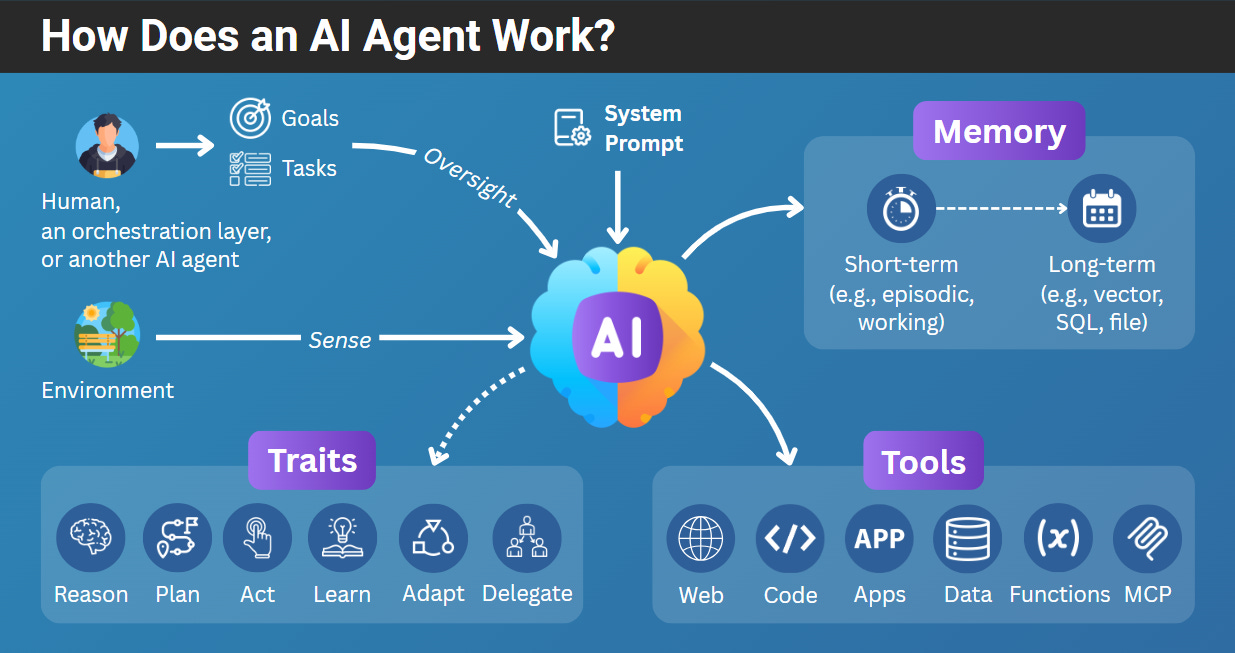
\includegraphics[width=\linewidth,keepaspectratio]{aiagents5}
	\end{center}
	
	{\tiny (Ref: The Ultimate Guide to AI Agents for PMs - Pawl Huryn)}
	
\end{frame}


%%%%%%%%%%%%%%%%%%%%%%%%%%%%%%%%%%%%%%%%%%%%%%%%%%%%%%%%%%%%%%%%%%%%%%%%%%%%%%%%%%
\begin{frame}[fragile]\frametitle{What Is an Agent? (Technical Definition)}
\begin{itemize}
    \item Agent acts and takes you from one state to another, providing value through workflow automation
    \item Based on ReAct paradigm: \textbf{Reasoning + Acting}
    \item Key capabilities:
    \begin{itemize}
        \item Can plan and make decisions
        \item Has access to tools (search APIs, booking, email, etc.)
        \item Interacts with external environments and other agents
        \item Maintains memory of conversations and actions
        \item May include human-in-the-loop for safety
    \end{itemize}
    \item Agents existed since the 1950s but are now effective because of LLMs
\end{itemize}
\end{frame}


%%%%%%%%%%%%%%%%%%%%%%%%%%%%%%%%%%%%%%%%%%%%%%%%%%%%%%%%%%%%%%%%%%%%%%%%%%%%%%%%%%
\begin{frame}[fragile]\frametitle{Two Ways to Define Agents}
\begin{columns}
    \begin{column}[T]{0.5\linewidth}
        \textbf{Technical View:}
        \begin{itemize}
            \item LLM (brain)
            \item + Tools (hands)
            \item + Planning (strategy)
            \item + Memory (context)
            \item + State management
        \end{itemize}
    \end{column}
    \begin{column}[T]{0.5\linewidth}
        \textbf{Business View:}
        \begin{itemize}
            \item Systems that complete tasks end-to-end
            \item Focus on outcomes, not components
            \item Solve real-world problems
            \item Provide measurable value
        \end{itemize}
    \end{column}
\end{columns}

\vspace{0.5cm}
\textbf{Important:} Today's agents are \textbf{engineering wrappers} around AI models, the intelligence comes from the LLMs, agents help act on that intelligence.
\end{frame}

%%%%%%%%%%%%%%%%%%%%%%%%%%%%%%%%%%%%%%%%%%%%%%%%%%%%%%%%%%%%%%%%%%%%%%%%%%%%%%%%%%
\begin{frame}[fragile]\frametitle{}
\begin{center}
{\Large Types of AI Agents}

{\tiny (Ref: Agentic AI For Everyone - Aish \& Kiriti)}
\end{center}
\end{frame}

%%%%%%%%%%%%%%%%%%%%%%%%%%%%%%%%%%%%%%%%%%%%%%%%%%%%%%%%%%%
\begin{frame}[fragile]\frametitle{The Tool-Augmented LLM}
    \begin{itemize}
        \item LLM is the brain of modern AI agents.
        \item Becomes agentic when paired with tools, planning, memory, and control logic.
        \item Enables reasoning, action-taking, and goal adaptation.
        \item Different autonomy levels define different agent types.
    \end{itemize}

\end{frame}


%%%%%%%%%%%%%%%%%%%%%%%%%%%%%%%%%%%%%%%%%%%%%%%%%%%%%%%%%%%
\begin{frame}[fragile]\frametitle{Rule-Based Systems}
    \begin{itemize}
        \item No LLM, just if-this-then-that logic.
        \item Best for simple, structured, repetitive tasks.
        \item Examples: auto-approvals, file renaming, data copying.
        \item Pros: Fast, predictable, auditable.
        \item Cons: Brittle, lacks flexibility or reasoning.
    \end{itemize}
\end{frame}

%%%%%%%%%%%%%%%%%%%%%%%%%%%%%%%%%%%%%%%%%%%%%%%%%%%%%%%%%%%
\begin{frame}[fragile]\frametitle{Workflow Agents}
    \begin{itemize}
        \item LLM assists but doesn't act independently.
        \item Human remains in control; agent augments tasks.
        \item Examples: email drafts, meeting summaries, query translation.
        \item Pros: Low risk, easy deployment, boosts productivity.
        \item Cons: No execution or planning capability.
    \end{itemize}
\end{frame}

%%%%%%%%%%%%%%%%%%%%%%%%%%%%%%%%%%%%%%%%%%%%%%%%%%%%%%%%%%%
\begin{frame}[fragile]\frametitle{Semi-Autonomous Agents}
    \begin{itemize}
        \item LLM plans and executes with limited supervision.
        \item Supports multi-step, tedious workflows.
        \item Examples: CRM outreach, contract data entry, research reports.
        \item Pros: Saves time, automates complex tasks.
        \item Cons: Needs infra (memory, tools), harder to test.
    \end{itemize}
\end{frame}

%%%%%%%%%%%%%%%%%%%%%%%%%%%%%%%%%%%%%%%%%%%%%%%%%%%%%%%%%%%
\begin{frame}[fragile]\frametitle{Autonomous Agents}
    \begin{itemize}
        \item Fully goal-driven, acts without oversight.
        \item Manages long-running, async, cross-system tasks.
        \item Examples: research briefs, ops monitoring, product testing.
        \item Pros: Highly scalable, handles complex goals.
        \item Cons: High risk, hard to monitor or trace.
    \end{itemize}
\end{frame}

%%%%%%%%%%%%%%%%%%%%%%%%%%%%%%%%%%%%%%%%%%%%%%%%%%%%%%%%%%%
\begin{frame}[fragile]\frametitle{Choosing the Right Agent Type}
    \begin{itemize}
        \item Start with the problem, not the tech.
        \item Key questions: structure, language needs, decision steps, human involvement.
        \item Use autonomy level as a design guide.
        \item Mix agent types if needed within one system.
    \end{itemize}
	
        \begin{center}
        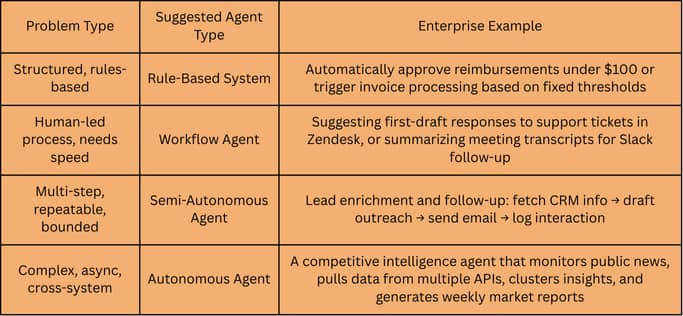
\includegraphics[width=0.8\linewidth,keepaspectratio]{aiagents3}
		
		{\tiny (Ref: Agentic AI For Everyone - Aish \& Kiriti)}
        \end{center}
		
\end{frame}

%%%%%%%%%%%%%%%%%%%%%%%%%%%%%%%%%%%%%%%%%%%%%%%%%%%%%%%%%%%
\begin{frame}[fragile]\frametitle{Keep in Mind \ldots}
    \begin{itemize}
        \item Problem requirements dictate agent design.
        \item Hybrid systems often work best in practice.
        \item Single or multi-agent setups depend on task complexity.
        \item Don't ask “How do I build an agent?” - ask “What problem am I solving?”
    \end{itemize}
\end{frame}


%%%%%%%%%%%%%%%%%%%%%%%%%%%%%%%%%%%%%%%%%%%%%%%%%%%%%%%%%%%%%%%%%%%%%%%%%%%%%%%%%%
\begin{frame}[fragile]\frametitle{Building Agentic AI: Start with Problems, Not Technology}
\begin{itemize}
    \item \textbf{Common mistake:} Starting with "Let's build an agent!"
    \item \textbf{Correct approach:} "What real-world problem are we solving?"
    \item Identify enterprise pain points first:
    \begin{itemize}
        \item Support teams drowning in repetitive queries
        \item Analysts switching between dashboards for insights
        \item Sales teams manually logging customer activity
    \end{itemize}
    \item Design choices matter for enterprise applications
    \item Focus on agents that work in the real world, not just demos
\end{itemize}
\end{frame}

%%%%%%%%%%%%%%%%%%%%%%%%%%%%%%%%%%%%%%%%%%%%%%%%%%%%%%%%%%%
\begin{frame}[fragile]\frametitle{Autonomy vs. Control: A Critical Trade-off}

		\begin{itemize}
			\item Key decision: How autonomous should your agent be?
			\item This is a \textbf{contextual trade-off}, not a one-size-fits-all decision
			\item Spectrum of autonomy:
			\begin{itemize}
				\item High human control ? Predictable, safe, limited capability
				\item High agent autonomy ? Flexible, powerful, potentially risky
			\end{itemize}
			\item Different problems demand different levels of agent involvement
			\item Consider: task complexity, risk tolerance, compliance requirements
		\end{itemize}

        \begin{center}
        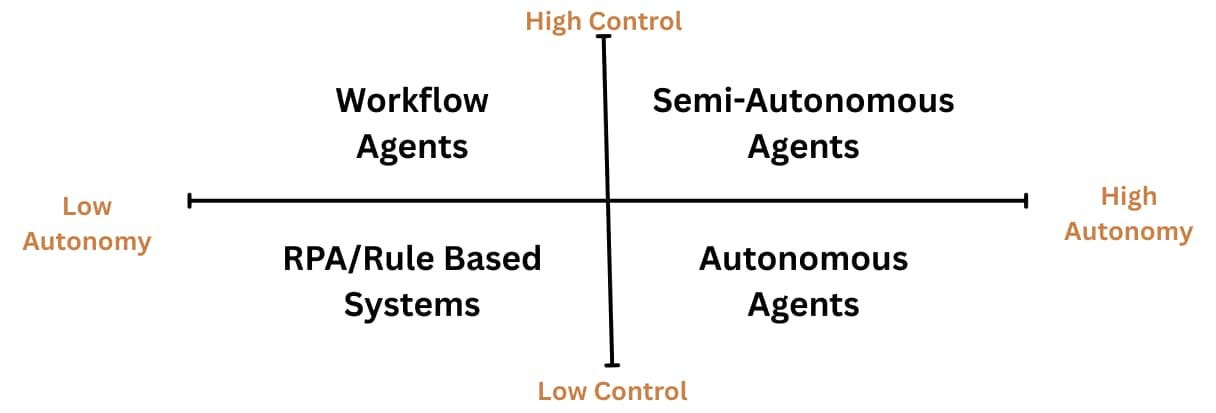
\includegraphics[width=0.8\linewidth,keepaspectratio]{aiagents2}
		
		{\tiny (Ref: Agentic AI For Everyone - Aish \& Kiriti)}
        \end{center}

\end{frame}


%%%%%%%%%%%%%%%%%%%%%%%%%%%%%%%%%%%%%%%%%%%%%%%%%%%%%%%%%%%%%%%%%%%%%%%%%%%%%%%%%%
\begin{frame}[fragile]\frametitle{When to Use Agents?}
\begin{itemize}
    \item \textbf{Best suited for:} Tasks requiring flexibility and model-driven decision-making
    \item \textbf{Consider trade-offs:} Agents increase latency and cost for better task performance
    \item \textbf{Recommended for:} Open-ended problems with unpredictable steps
    \item \textbf{Simple solutions preferred:} Single LLM calls with retrieval often sufficient
    \item Agents are systems where LLMs dynamically direct their own processes and tool usage
    \item Can operate autonomously over extended periods using various tools
    \item Distinct from workflows: agents have dynamic control vs. predefined code paths
\end{itemize}
\end{frame}

%%%%%%%%%%%%%%%%%%%%%%%%%%%%%%%%%%%%%%%%%%%%%%%%%%%%%%%%%%%
\begin{frame}[fragile]\frametitle{What is an AI Agent?}
    \begin{itemize}
        \item Autonomous software for single task execution.
        \item Triggered by prompts; performs within defined scope.
        \item May include optional memory or tool cache.
        \item Examples: email filtering, scheduling, internal search.
        \item Behaves like a thermostat—limited but precise.
    \end{itemize}
\end{frame}

%%%%%%%%%%%%%%%%%%%%%%%%%%%%%%%%%%%%%%%%%%%%%%%%%%%%%%%%%%%
\begin{frame}[fragile]\frametitle{What is Agentic AI?}
    \begin{itemize}
        \item Involves multiple agents collaborating dynamically.
        \item Goal-based initiation and task decomposition.
        \item Shares context and episodic memory among agents.
        \item Learns from outcomes to refine strategy.
        \item Examples: research assistants, robotics, adaptive AI.
        \item Acts like a smart control center—coordinated and adaptive.
    \end{itemize}
\end{frame}

%%%%%%%%%%%%%%%%%%%%%%%%%%%%%%%%%%%%%%%%%%%%%%%%%%%%%%%%%%%
\begin{frame}[fragile]\frametitle{Functional Domains}
    \begin{itemize}
        \item \textbf{AI Agents:} Internal search, email sorting, scheduling.
        \item \textbf{Agentic AI:} Multi-agent research, game AI, robotics.
        \item Domains defined by complexity and inter-agent coordination.
    \end{itemize}
\end{frame}

%%%%%%%%%%%%%%%%%%%%%%%%%%%%%%%%%%%%%%%%%%%%%%%%%%%%%%%%%%%
\begin{frame}[fragile]\frametitle{Architectural Evolution}
    \begin{itemize}
        \item \textbf{AI Agent:} Perception → Reasoning → Action.
        \item \textbf{Agentic AI:} Agents + Shared context + Memory + Collaboration.
        \item Evolution toward orchestration and persistent context.
        \item Future: Dynamic, memory-rich, goal-oriented systems.
    \end{itemize}
\end{frame}

%%%%%%%%%%%%%%%%%%%%%%%%%%%%%%%%%%%%%%%%%%%%%%%%%%%%%%%%%%%
\begin{frame}[fragile]\frametitle{Core Differences Overview}
\begin{tabular}{|l|l|l|}
\hline
\textbf{Aspect} & \textbf{AI Agent} & \textbf{Agentic AI} \\
\hline
Trigger & Prompt-based & Goal-based \\
Flexibility & Fixed scope & Adaptive system \\
Memory & Optional cache & Shared episodic memory \\
Learning & Minimal tweaking & Learns from outcomes \\
Coordination & Single-agent & Multi-agent collaboration \\
\hline
\end{tabular}
\end{frame}

%%%%%%%%%%%%%%%%%%%%%%%%%%%%%%%%%%%%%%%%%%%%%%%%%%%%%%%%%%%
\begin{frame}[fragile]\frametitle{Evolving Landscape}
    \begin{itemize}
        \item AI Agents now support multi-agent protocols (e.g., MCP, A2A).
        \item Expanded tool usage and dynamic collaboration features.
        \item Blurring lines between AI Agents and Agentic AI.
        \item Functional memory increasingly common in AI Agents.
        \item Agentic principles gradually adopted in modern agents.
    \end{itemize}
\end{frame}



%%%%%%%%%%%%%%%%%%%%%%%%%%%%%%%%%%%%%%%%%%%%%%%%%%%%%%%%%%%%%%%%%%%%%%%%%%%%%%%%%%
\begin{frame}[fragile]\frametitle{}
\begin{center}
{\Large Agent Architecture Patterns}
\end{center}
\end{frame}

%%%%%%%%%%%%%%%%%%%%%%%%%%%%%%%%%%%%%%%%%%%%%%%%%%%%%%%%%%%%%%%%%%%%%%%%%%%%%%%%%%
\begin{frame}[fragile]\frametitle{Building Block: Augmented LLM}
\begin{itemize}
    \item Foundation of agentic systems
    \item Enhanced with retrieval, tools, and memory capabilities
    \item Can generate search queries independently
    \item Actively selects appropriate tools and determines information retention
\end{itemize}

\begin{center}
\includegraphics[width=\linewidth,keepaspectratio]{finetune9}
\end{center}

{\tiny (Ref: Building effective agents - Anthropic)}
\end{frame}

%%%%%%%%%%%%%%%%%%%%%%%%%%%%%%%%%%%%%%%%%%%%%%%%%%%%%%%%%%%%%%%%%%%%%%%%%%%%%%%%%%
\begin{frame}[fragile]\frametitle{Workflow Pattern: Prompt Chaining}
\begin{itemize}
    \item Decomposes tasks into sequential steps
    \item Each LLM call processes previous output
    \item Includes programmatic checks for process verification
    \item Ideal for tasks with clear, fixed subtasks
    \item Examples: Marketing copy generation and translation, document outline creation
\end{itemize}

\begin{center}
\includegraphics[width=\linewidth,keepaspectratio]{finetune10}
\end{center}

{\tiny (Ref: Building effective agents - Anthropic)}
\end{frame}

%%%%%%%%%%%%%%%%%%%%%%%%%%%%%%%%%%%%%%%%%%%%%%%%%%%%%%%%%%%%%%%%%%%%%%%%%%%%%%%%%%
\begin{frame}[fragile]\frametitle{Workflow Pattern: Routing}
\begin{itemize}
    \item Classifies input and directs to specialized follow-up tasks
    \item Enables separation of concerns and specialized prompts
    \item Suitable for complex tasks with distinct categories
    \item Applications: Customer service query distribution, model optimization based on query complexity
\end{itemize}

\begin{center}
\includegraphics[width=\linewidth,keepaspectratio]{finetune11}
\end{center}

{\tiny (Ref: Building effective agents - Anthropic)}
\end{frame}

%%%%%%%%%%%%%%%%%%%%%%%%%%%%%%%%%%%%%%%%%%%%%%%%%%%%%%%%%%%%%%%%%%%%%%%%%%%%%%%%%%
\begin{frame}[fragile]\frametitle{Workflow Pattern: Parallelization}
\begin{itemize}
    \item Two key variations: Sectioning and Voting
    \item \textbf{Sectioning:} Breaks tasks into parallel subtasks
    \item \textbf{Voting:} Runs same task multiple times for diverse outputs
    \item Effective for speed optimization and confidence improvement
    \item Use cases: Content screening, code vulnerability review
\end{itemize}

\begin{center}
\includegraphics[width=\linewidth,keepaspectratio]{finetune12}
\end{center}

{\tiny (Ref: Building effective agents - Anthropic)}
\end{frame}

%%%%%%%%%%%%%%%%%%%%%%%%%%%%%%%%%%%%%%%%%%%%%%%%%%%%%%%%%%%%%%%%%%%%%%%%%%%%%%%%%%
\begin{frame}[fragile]\frametitle{Workflow Pattern: Orchestrator-Workers}
\begin{itemize}
    \item Central LLM coordinates task breakdown and delegation
    \item Dynamically determines subtasks based on input
    \item Suitable for complex, unpredictable task structures
    \item Applications: Multi-file code changes, comprehensive information gathering
\end{itemize}

\begin{center}
\includegraphics[width=\linewidth,keepaspectratio]{finetune13}
\end{center}

{\tiny (Ref: Building effective agents - Anthropic)}
\end{frame}

%%%%%%%%%%%%%%%%%%%%%%%%%%%%%%%%%%%%%%%%%%%%%%%%%%%%%%%%%%%%%%%%%%%%%%%%%%%%%%%%%%
\begin{frame}[fragile]\frametitle{Workflow Pattern: Evaluator-Optimizer}
\begin{itemize}
    \item One LLM generates, another evaluates in a feedback loop
    \item Effective with clear evaluation criteria
    \item Ideal for iterative refinement processes
    \item Examples: Literary translation, complex search tasks
\end{itemize}

\begin{center}
\includegraphics[width=\linewidth,keepaspectratio]{finetune14}
\end{center}

{\tiny (Ref: Building effective agents - Anthropic)}
\end{frame}

%%%%%%%%%%%%%%%%%%%%%%%%%%%%%%%%%%%%%%%%%%%%%%%%%%%%%%%%%%%%%%%%%%%%%%%%%%%%%%%%%%
\begin{frame}[fragile]\frametitle{}
\begin{center}
{\Large Agent Autonomy Levels}
\end{center}
\end{frame}

%%%%%%%%%%%%%%%%%%%%%%%%%%%%%%%%%%%%%%%%%%%%%%%%%%%%%%%%%%%%%%%%%%%%%%%%%%%%%%%%%%
\begin{frame}[fragile]\frametitle{AI Agent Levels Overview}
\begin{itemize}
    \item Hugging Face defines 5 levels of AI agents
    \item Based on autonomy in decision-making and execution
    \item Control shifts from human to system as levels increase
    \item From paper: "Fully Autonomous AI Agents Should Not be Developed"
    \item This framework clarifies much-needed concepts about autonomy in AI agents
\end{itemize}
\end{frame}

%%%%%%%%%%%%%%%%%%%%%%%%%%%%%%%%%%%%%%%%%%%%%%%%%%%%%%%%%%%%%%%%%%%%%%%%%%%%%%%%%%
\begin{frame}[fragile]\frametitle{Level 1 - Simple Processor}
\begin{itemize}
    \item No impact on program flow
    \item Direct input-output processing
    \item Example: Printing LLM output
    \item Control: Fully human-driven
    \item Most basic form of AI integration
\end{itemize}
\end{frame}

%%%%%%%%%%%%%%%%%%%%%%%%%%%%%%%%%%%%%%%%%%%%%%%%%%%%%%%%%%%%%%%%%%%%%%%%%%%%%%%%%%
\begin{frame}[fragile]\frametitle{Level 2 - Router}
\begin{itemize}
    \item Determines basic program flow
    \item Routes execution based on conditions
    \item Example: If-else decision logic
    \item Control: Human (how), System (when)
    \item First level where AI influences execution path
\end{itemize}
\end{frame}

%%%%%%%%%%%%%%%%%%%%%%%%%%%%%%%%%%%%%%%%%%%%%%%%%%%%%%%%%%%%%%%%%%%%%%%%%%%%%%%%%%
\begin{frame}[fragile]\frametitle{Level 3 - Tool Calling}
\begin{itemize}
    \item Determines how functions execute
    \item Chooses tools and parameters dynamically
    \item Example: Running LLM-chosen tools
    \item Control: Human (what), System (how)
    \item This is where most current "agents" operate
\end{itemize}
\end{frame}

%%%%%%%%%%%%%%%%%%%%%%%%%%%%%%%%%%%%%%%%%%%%%%%%%%%%%%%%%%%%%%%%%%%%%%%%%%%%%%%%%%
\begin{frame}[fragile]\frametitle{Level 4 - Multi-Step Agent}
\begin{itemize}
    \item Controls iteration and continuation
    \item Executes multi-step workflows
    \item Example: Looping task execution
    \item Control: Human (what), System (which, when, how)
    \item Significant autonomy with human goal-setting
\end{itemize}
\end{frame}

%%%%%%%%%%%%%%%%%%%%%%%%%%%%%%%%%%%%%%%%%%%%%%%%%%%%%%%%%%%%%%%%%%%%%%%%%%%%%%%%%%
\begin{frame}[fragile]\frametitle{Level 5 - Fully Autonomous Agent}
\begin{itemize}
    \item Creates and executes new code
    \item Generates, validates, and runs programs
    \item Example: Code generation from user request
    \item Control: Fully system-driven
    \item \textbf{Warning:} Hugging Face argues these should not be developed
\end{itemize}
\end{frame}

%%%%%%%%%%%%%%%%%%%%%%%%%%%%%%%%%%%%%%%%%%%%%%%%%%%%%%%%%%%%%%%%%%%%%%%%%%%%%%%%%%
\begin{frame}[fragile]\frametitle{Agent Levels Summary}
\begin{center}
\includegraphics[width=0.8\linewidth,keepaspectratio]{agents_levels}
\end{center}

{\tiny (Ref: LinkedIn post - Rakesh Gohel)}
\end{frame}


%%%%%%%%%%%%%%%%%%%%%%%%%%%%%%%%%%%%%%%%%%%%%%%%%%%%%%%%%%%%%%%%%%%%%%%%%%%%%%%%%%
\begin{frame}[fragile]\frametitle{}
\begin{center}
{\Large Real-World Agentic Systems}

{\tiny (Ref: Agentic AI For Everyone - Aish \& Kiriti)}
\end{center}
\end{frame}

%%%%%%%%%%%%%%%%%%%%%%%%%%%%%%%%%%%%%%%%%%%%%%%%%%%%%%%%%%%%%%%%%%%%%%%%%%%%%%%%%%
\begin{frame}[fragile]\frametitle{Agentic Systems Overview}
    \begin{itemize}
        \item Agentic systems exhibit goal-directed, multi-step behavior.
        \item Focus is on three systems: NotebookLM, Perplexity, DeepResearch.
        \item These aren't open-source; analysis is based on observed behavior.
        \item All rely on planning, retrieval (RAG), memory, and tool use.
        \item Their behavior varies in level of autonomy and task complexity.
    \end{itemize}
\end{frame}

%%%%%%%%%%%%%%%%%%%%%%%%%%%%%%%%%%%%%%%%%%%%%%%%%%%%%%%%%%%%%%%%%%%%%%%%%%%%%%%%%%
\begin{frame}[fragile]\frametitle{NotebookLM: Personal Research Assistant}
    \begin{itemize}
        \item Users upload files like PDFs, notes, slides.
        \item Files are preprocessed for retrieval-based tasks.
        \item Supports summarizing, Q&A, audio creation, guides.
        \item Determines task type: summary, Q&A, comparison, etc.
        \item Uses RAG to find and use relevant document sections.
        \item Generates answers grounded in user data.
        \item Short-term memory tracks conversation flow.
        \item Limited or no long-term memory.
        \item Tools may include viewers and summarizers.
    \end{itemize}
\end{frame}

%%%%%%%%%%%%%%%%%%%%%%%%%%%%%%%%%%%%%%%%%%%%%%%%%%%%%%%%%%%%%%%%%%%%%%%%%%%%%%%%%%
\begin{frame}[fragile]\frametitle{Why NotebookLM is Agentic}
    \begin{itemize}
        \item Understands user intent, not just input.
        \item Selects relevant parts of user-uploaded data.
        \item Responds in structured, meaningful formats.
        \item Behaves like a goal-oriented assistant.
        \item Operates as a high-control workflow agent.
        \item Falls between level 2 and level 3 autonomy.
    \end{itemize}
\end{frame}

%%%%%%%%%%%%%%%%%%%%%%%%%%%%%%%%%%%%%%%%%%%%%%%%%%%%%%%%%%%%%%%%%%%%%%%%%%%%%%%%%%
\begin{frame}[fragile]\frametitle{Perplexity: Web-Based Q\&A Agent}
    \begin{itemize}
        \item Accepts user questions on open-ended topics.
        \item Plans searches based on query semantics.
        \item Uses web search APIs to gather data.
        \item Applies RAG to find credible content.
        \item Synthesizes direct answers with citations.
        \item Maintains short-term context memory.
        \item May adapt to user preferences long-term.
    \end{itemize}
\end{frame}

%%%%%%%%%%%%%%%%%%%%%%%%%%%%%%%%%%%%%%%%%%%%%%%%%%%%%%%%%%%%%%%%%%%%%%%%%%%%%%%%%%
\begin{frame}[fragile]\frametitle{Why Perplexity is Agentic}
    \begin{itemize}
        \item Interprets intent and makes decisions.
        \item Chooses tools and content autonomously.
        \item Constructs coherent answers from sources.
        \item Demonstrates multi-step reasoning.
        \item Closer to level 3, possibly level 4 agent.
        \item User delegates task, not just assists.
    \end{itemize}
\end{frame}

%%%%%%%%%%%%%%%%%%%%%%%%%%%%%%%%%%%%%%%%%%%%%%%%%%%%%%%%%%%%%%%%%%%%%%%%%%%%%%%%%%
\begin{frame}[fragile]\frametitle{DeepResearch: Advanced Task Automation}
    \begin{itemize}
        \item Designed for complex, open-ended tasks.
        \item Breaks big questions into subtasks.
        \item Plans multi-step research workflows.
        \item Integrates tools: search, readers, graphs.
        \item Uses agentic RAG: reflect, refetch, revise.
        \item Tracks task progress with episodic memory.
        \item Stores key insights with semantic memory.
    \end{itemize}
\end{frame}

%%%%%%%%%%%%%%%%%%%%%%%%%%%%%%%%%%%%%%%%%%%%%%%%%%%%%%%%%%%%%%%%%%%%%%%%%%%%%%%%%%
\begin{frame}[fragile]\frametitle{Why DeepResearch is Agentic}
    \begin{itemize}
        \item Performs deep, self-driven analysis.
        \item Operates through iterative agent loops.
        \item Executes plans with minimal user guidance.
        \item Demonstrates high independence and adaptability.
        \item Behaves like a strong level 4 agent.
    \end{itemize}
\end{frame}

%%%%%%%%%%%%%%%%%%%%%%%%%%%%%%%%%%%%%%%%%%%%%%%%%%%%%%%%%%%%%%%%%%%%%%%%%%%%%%%%%%
\begin{frame}[fragile]\frametitle{Comparing Agentic Levels}
    \begin{itemize}
        \item NotebookLM: Level 2–3, guided step-by-step.
        \item Perplexity: Level 3–4, plans and answers autonomously.
        \item DeepResearch: Strong Level 4, drives complex tasks.
        \item Key components: planning, RAG, memory, tools.
        \item Main difference: how much control system has vs. user.
    \end{itemize}
\end{frame}

%%%%%%%%%%%%%%%%%%%%%%%%%%%%%%%%%%%%%%%%%%%%%%%%%%%%%%%%%%%%%%%%%%%%%%%%%%%%%%%%%%
\begin{frame}[fragile]\frametitle{}
\begin{center}
{\Large Agentic RAG}

{\tiny (Ref: LinkedIn post by Rakesh Gohel)}

\end{center}
\end{frame}

%%%%%%%%%%%%%%%%%%%%%%%%%%%%%%%%%%%%%%%%%%%%%%%%%%%%%%%%%%%%%%%%%%%%%%%%%%%%%%%%%%
\begin{frame}[fragile]\frametitle{Agentic RAG in 2025}
    \begin{itemize}
        \item RAG (Retrieval Augmented Generation) remains vital in 2025.
        \item Used by systems like Glean AI, Perplexity, Harvey.
        \item Combines RAG with AI agents for enterprise workflows.
        \item Enables dynamic, multi-step reasoning and data use.
        \item Ideal for handling complex business queries.
    \end{itemize}
\end{frame}

%%%%%%%%%%%%%%%%%%%%%%%%%%%%%%%%%%%%%%%%%%%%%%%%%%%%%%%%%%%%%%%%%%%%%%%%%%%%%%%%%%
\begin{frame}[fragile]\frametitle{RAG: Retrieval-Augmented Generation}
    \begin{itemize}
        \item \textbf{Query \& Embedding:} Retrieves data via vector search.
        \item \textbf{Vector DB:} Extracts info from pre-indexed embeddings.
        \item \textbf{Prompt Addition:} Combines retrieved data with query.
        \item \textbf{LLM Generation:} Final response is produced by LLM.
        \item Provides grounded, context-aware outputs.
    \end{itemize}
\end{frame}

%%%%%%%%%%%%%%%%%%%%%%%%%%%%%%%%%%%%%%%%%%%%%%%%%%%%%%%%%%%%%%%%%%%%%%%%%%%%%%%%%%
\begin{frame}[fragile]\frametitle{AI Agents in the Workflow}
    \begin{itemize}
        \item \textbf{Query Handling:} Analyzes the user’s intent.
        \item \textbf{Planning \& Memory:} Uses ReAct/Reflexion for strategy.
        \item \textbf{Tool Usage:} Pulls live data using external APIs.
        \item \textbf{Response:} Synthesizes answer using all retrieved info.
        \item Adds reasoning and dynamic task execution.
    \end{itemize}
\end{frame}

%%%%%%%%%%%%%%%%%%%%%%%%%%%%%%%%%%%%%%%%%%%%%%%%%%%%%%%%%%%%%%%%%%%%%%%%%%%%%%%%%%
\begin{frame}[fragile]\frametitle{Combining RAG with AI Agents}
    \begin{itemize}
        \item AI agents manage embedding and data source selection.
        \item Use RAG’s retrieval to gather relevant information.
        \item Enhance RAG prompts with planning and real-time data.
        \item Result: More accurate and context-rich responses.
        \item Allows scalable and adaptive workflows.
    \end{itemize}
\end{frame}

%%%%%%%%%%%%%%%%%%%%%%%%%%%%%%%%%%%%%%%%%%%%%%%%%%%%%%%%%%%%%%%%%%%%%%%%%%%%%%%%%%
\begin{frame}[fragile]\frametitle{Operational Workflow Overview}
    \begin{itemize}
        \item \textbf{1. Query Routing:} Directed to agent for orchestration.
        \item \textbf{2. Context Retention:} Memory tracks user session.
        \item \textbf{3. Task Planning:} Defines strategy and tools needed.
        \item \textbf{4. Data Fetching:} Pulls from knowledge base via tools.
        \item \textbf{5. Prompt Optimisation:} Combines, reasons, prepares input.
        \item \textbf{6. Response Generation:} LLM finalizes and outputs answer.
    \end{itemize}
\end{frame}

%%%%%%%%%%%%%%%%%%%%%%%%%%%%%%%%%%%%%%%%%%%%%%%%%%%%%%%%%%%
\begin{frame}[fragile]\frametitle{}

\begin{center}
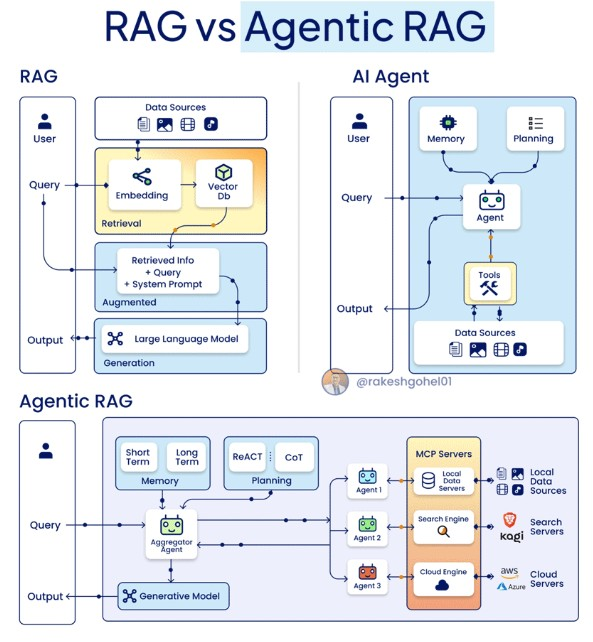
\includegraphics[width=0.6\linewidth,keepaspectratio]{aiagents23}
\end{center}	  
\end{frame}


%%%%%%%%%%%%%%%%%%%%%%%%%%%%%%%%%%%%%%%%%%%%%%%%%%%%%%%%%%%%%%%%%%%%%%%%%%%%%%%%%%
\begin{frame}[fragile]\frametitle{}
\begin{center}
{\Large From Monolithic to Compound AI}
\end{center}
\end{frame}

%%%%%%%%%%%%%%%%%%%%%%%%%%%%%%%%%%%%%%%%%%%%%%%%%%%%%%%%%%%%%%%%%%%%%%%%%%%%%%%%%%
\begin{frame}[fragile]\frametitle{From Monolithic Models to Compound AI}
\begin{itemize}
    \item \textbf{Monolithic models} are limited by training data
    \item Hard to adapt without significant data and resources
    \item Example: Vacation planning with no access to personal data
    \item \textbf{Compound AI systems} solve this by integrating multiple components
    \item External databases and tools enhance model responses
    \item Shifting from single models to integrated AI systems
\end{itemize}
\end{frame}

%%%%%%%%%%%%%%%%%%%%%%%%%%%%%%%%%%%%%%%%%%%%%%%%%%%%%%%%%%%%%%%%%%%%%%%%%%%%%%%%%%
\begin{frame}[fragile]\frametitle{System Design in Compound AI}
\begin{itemize}
    \item Systems are modular: combine models, tools, and databases
    \item Easier to adapt and quicker to solve problems
    \item Combining models with external components for enhanced output
    \item Example: Search query integrated with model for better accuracy
    \item Programmatic control logic guides the response
    \item Compound AI systems use system design for better problem-solving
\end{itemize}
\end{frame}

%%%%%%%%%%%%%%%%%%%%%%%%%%%%%%%%%%%%%%%%%%%%%%%%%%%%%%%%%%%%%%%%%%%%%%%%%%%%%%%%%%
\begin{frame}[fragile]\frametitle{Role of Agents in Compound AI}
\begin{itemize}
    \item Agents use large language models (LLMs) for reasoning and planning
    \item LLMs break down problems into manageable tasks
    \item Slow thinking (planning) leads to better solutions
    \item Agents provide flexibility in solving complex tasks
    \item The agent's role is to manage logic and interact with tools
    \item AI agents improve with reasoning, acting, and memory components
\end{itemize}
\end{frame}

%%%%%%%%%%%%%%%%%%%%%%%%%%%%%%%%%%%%%%%%%%%%%%%%%%%%%%%%%%%%%%%%%%%%%%%%%%%%%%%%%%
\begin{frame}[fragile]\frametitle{Components of LLM Agents}
\begin{itemize}
    \item \textbf{Reasoning:} Break down complex problems into steps
    \item \textbf{Acting:} Use external tools like databases or calculators
    \item \textbf{Memory:} Store logs and conversation history for personalization
    \item \textbf{Tools:} External programs that help solve problems (search, calculators)
    \item \textbf{Configurations:} Adjust agents using frameworks like ReAct
    \item Enhanced with planning modules and state management
\end{itemize}
\end{frame}

%%%%%%%%%%%%%%%%%%%%%%%%%%%%%%%%%%%%%%%%%%%%%%%%%%%%%%%%%%%%%%%%%%%%%%%%%%%%%%%%%%
\begin{frame}[fragile]\frametitle{Example: ReAct Agent in Action}
\begin{itemize}
    \item ReAct agents think slowly, plan, and act iteratively
    \item User query feeds into the agent with reasoning instructions
    \item The agent may call external tools and evaluate the results
    \item If the result is wrong, the agent revises its plan
    \item Example: Calculating sunscreen needs for a vacation
    \item Demonstrates the power of reasoning + acting paradigm
\end{itemize}
\end{frame}

%%%%%%%%%%%%%%%%%%%%%%%%%%%%%%%%%%%%%%%%%%%%%%%%%%%%%%%%%%%%%%%%%%%%%%%%%%%%%%%%%%
\begin{frame}[fragile]\frametitle{Agent Autonomy in Problem Solving}
\begin{itemize}
    \item Narrow problems can be solved with fixed, programmatic systems
    \item Complex tasks require agent autonomy for better flexibility
    \item Autonomy level depends on task complexity and need for iteration
    \item Agents are effective for complex, diverse tasks (e.g., GitHub issues)
    \item Modular AI systems can solve more complex problems
    \item Example: Planning vacation with weather, sunscreen, and health data
\end{itemize}
\end{frame}

%%%%%%%%%%%%%%%%%%%%%%%%%%%%%%%%%%%%%%%%%%%%%%%%%%%%%%%%%%%%%%%%%%%%%%%%%%%%%%%%%%
\begin{frame}[fragile]\frametitle{}
\begin{center}
{\Large Agents in Production}
\end{center}
\end{frame}

%%%%%%%%%%%%%%%%%%%%%%%%%%%%%%%%%%%%%%%%%%%%%%%%%%%%%%%%%%%%%%%%%%%%%%%%%%%%%%%%%%
\begin{frame}[fragile]\frametitle{Agents in Production}
\begin{itemize}
    \item Operate independently with human interaction when needed
    \item Require environmental feedback for progress assessment
    \item Implementation often straightforward despite sophistication
    \item Key applications: SWE-bench tasks, computer use automation
    \item Important considerations: Cost management and error prevention
\end{itemize}

\begin{center}
\includegraphics[width=\linewidth,keepaspectratio]{finetune15}
\end{center}

{\tiny (Ref: Building effective agents - Anthropic)}
\end{frame}

%%%%%%%%%%%%%%%%%%%%%%%%%%%%%%%%%%%%%%%%%%%%%%%%%%%%%%%%%%%%%%%%%%%%%%%%%%%%%%%%%%
\begin{frame}[fragile]\frametitle{High-Level Flow of a Coding Agent}
\begin{center}
\includegraphics[width=\linewidth,keepaspectratio]{finetune16}
\end{center}

{\tiny (Ref: Building effective agents - Anthropic)}
\end{frame}

%%%%%%%%%%%%%%%%%%%%%%%%%%%%%%%%%%%%%%%%%%%%%%%%%%%%%%%%%%%%%%%%%%%%%%%%%%%%%%%%%%
\begin{frame}[fragile]\frametitle{Examples of Agentic AI}
\begin{itemize}
    \item Agents mean \textbf{ACTION}
    \item Agentic AI means \textbf{ACTION using AI} (specifically LLMs)
    \item Examples across domains:
    \begin{itemize}
        \item \textbf{Personal assistants:} Calendar management, email automation
        \item \textbf{Autonomous robots:} Physical world interaction
        \item \textbf{Gaming agents:} Strategic decision-making
        \item \textbf{Science agents:} Research and experimentation
        \item \textbf{Web agents:} Browser automation, data collection
        \item \textbf{Software agents:} Code generation, debugging
    \end{itemize}
\end{itemize}
\end{frame}

%%%%%%%%%%%%%%%%%%%%%%%%%%%%%%%%%%%%%%%%%%%%%%%%%%%%%%%%%%%%%%%%%%%%%%%%%%%%%%%%%%
\begin{frame}[fragile]\frametitle{Autonomous AI Agents: The Collaborative Advantage}
\begin{itemize}
    \item Collaborative approach yields astonishing enhancements in performance
    \item Contrasted with using a single AI (like ChatGPT) in isolation
    \item Ability to assume distinct roles within a team
    \item Like professionals in various fields
    \item Each agent contributes specialized expertise to the conversation
    \item Multi-agent systems outperform single-agent approaches
\end{itemize}
\end{frame}

%%%%%%%%%%%%%%%%%%%%%%%%%%%%%%%%%%%%%%%%%%%%%%%%%%%%%%%%%%%%%%%%%%%%%%%%%%%%%%%%%%
\begin{frame}[fragile]\frametitle{The Agent Blueprint}
\begin{itemize}
    \item \textbf{Planning:} Reflects on past experiences, offers self-critiques, and breaks down tasks using sub-goal decomposition
    \item \textbf{Memory:} Utilizes sensory, short-term, and long-term memory for:
    \begin{itemize}
        \item Real-time data processing
        \item Task-specific information
        \item Retaining knowledge and experiences
    \end{itemize}
    \item \textbf{Tools:} Equipped with a virtual toolbox accessing calendars, calculators, search engines, and other resources for versatile problem-solving
\end{itemize}
\end{frame}

%%%%%%%%%%%%%%%%%%%%%%%%%%%%%%%%%%%%%%%%%%%%%%%%%%%%%%%%%%%%%%%%%%%%%%%%%%%%%%%%%%
\begin{frame}[fragile]\frametitle{Agent Flow: The Symphony}
\begin{itemize}
    \item \textbf{Task Decomposition:} Breaks down tasks into smaller, manageable components
    \item \textbf{Model (LLM) Selection:} Chooses the most suitable LLM for the task
    \item \textbf{Task Execution:} Leveraging planning, memory, and tools
    \item \textbf{Response Generation:} Creates contextually relevant and accurate responses
    \begin{itemize}
        \item Drafting reports
        \item Answering questions
        \item Making decisions
    \end{itemize}
\end{itemize}
\end{frame}

%%%%%%%%%%%%%%%%%%%%%%%%%%%%%%%%%%%%%%%%%%%%%%%%%%%%%%%%%%%%%%%%%%%%%%%%%%%%%%%%%%
\begin{frame}[fragile]\frametitle{}
\begin{center}
{\Large Agentic Frameworks}
\end{center}
\end{frame}

%%%%%%%%%%%%%%%%%%%%%%%%%%%%%%%%%%%%%%%%%%%%%%%%%%%%%%%%%%%%%%%%%%%%%%%%%%%%%%%%%%
\begin{frame}[fragile]\frametitle{Frameworks and Implementation}
\begin{itemize}
    \item Popular frameworks: LangGraph from LangChain, Amazon Bedrock AI Agent
    \item Start with direct LLM APIs - many patterns need just a few lines of code
    \item Frameworks can obscure underlying prompts and responses
    \item Understanding the underlying code is crucial for effective implementation
    \item Choose framework based on specific needs and complexity requirements
\end{itemize}
\end{frame}

%%%%%%%%%%%%%%%%%%%%%%%%%%%%%%%%%%%%%%%%%%%%%%%%%%%%%%%%%%%%%%%%%%%%%%%%%%%%%%%%%%
\begin{frame}[fragile]\frametitle{Agentic Framework Requirements}
\begin{itemize}
    \item \textbf{Intuitive unified agentic abstraction}
    \item \textbf{Flexible multi-agent orchestration}
    \item \textbf{Effective implementation of agentic design patterns}
    \item \textbf{Support diverse application needs:}
    \begin{itemize}
        \item Handle more complex tasks and improve response quality
        \item Easy to understand, maintain, and extend
        \item Modular composition with natural human participation
        \item Fast and creative experimentation
    \end{itemize}
    \item \textbf{Agentic Abstraction:} Unify models, tools, humans for compound AI systems
\end{itemize}
\end{frame}

%%%%%%%%%%%%%%%%%%%%%%%%%%%%%%%%%%%%%%%%%%%%%%%%%%%%%%%%%%%%%%%%%%%%%%%%%%%%%%%%%%
\begin{frame}[fragile]\frametitle{Multi-Agent Orchestration}
\begin{columns}
    \begin{column}[T]{0.6\linewidth}
        \begin{itemize}
            \item \textbf{Static/Dynamic:} Pre-defined vs. adaptive workflows
            \item \textbf{Context sharing/Isolation:} Information flow control
            \item \textbf{Cooperation/Competition:} Collaborative vs. competitive dynamics
            \item \textbf{Centralized/Decentralized:} Control structure design
            \item \textbf{Intervention/Automation:} Human involvement level
        \end{itemize}
    \end{column}
    \begin{column}[T]{0.4\linewidth}
        \begin{center}
        \includegraphics[width=\linewidth,keepaspectratio]{autoagent4}
        \end{center}
    \end{column}
\end{columns}
\end{frame}

%%%%%%%%%%%%%%%%%%%%%%%%%%%%%%%%%%%%%%%%%%%%%%%%%%%%%%%%%%%%%%%%%%%%%%%%%%%%%%%%%%
\begin{frame}[fragile]\frametitle{Popular Agentic Frameworks}
\begin{itemize}
    \item \textbf{BabyAGI:} Pioneering AI learning system
    \item \textbf{AutoGPT:} Automates content generation
    \item \textbf{GPT Engineer:} Assists in coding and software development
    \item \textbf{LangGraph:} Graph-based control flow
    \item \textbf{CrewAI:} High-level static agent-task workflow
    \item \textbf{AutoGen:} Dialog-based planning and execution
\end{itemize}
\end{frame}

%%%%%%%%%%%%%%%%%%%%%%%%%%%%%%%%%%%%%%%%%%%%%%%%%%%%%%%%%%%%%%%%%%%%%%%%%%%%%%%%%%
\begin{frame}[fragile]\frametitle{LangGraph}
\begin{itemize}
    \item Open-source framework by \textbf{LangChain} for stateful, multi-actor applications
    \item Inspired by \textbf{directed acyclic graphs (DAGs)} for data processing pipelines
    \item Treats workflows as graphs with \textbf{nodes for specific tasks or functions}
    \item Enables \textbf{fine-grained control} over application flow and state
    \item Suitable for \textbf{complex workflows} with advanced memory and error recovery
    \item Supports \textbf{human-in-the-loop} interactions
    \item Integrates with \textbf{LangChain} for tools and models
    \item Supports \textbf{multi-agent interaction patterns}
\end{itemize}
\end{frame}

%%%%%%%%%%%%%%%%%%%%%%%%%%%%%%%%%%%%%%%%%%%%%%%%%%%%%%%%%%%%%%%%%%%%%%%%%%%%%%%%%%
\begin{frame}[fragile]\frametitle{AutoGen}
\begin{itemize}
    \item Framework by \textbf{Microsoft} for building conversational agents
    \item Treats workflows as \textbf{conversations between agents}
    \item Intuitive for users preferring \textbf{ChatGPT-like interfaces}
    \item Supports tools like \textbf{code executors} and \textbf{function callers}
    \item Allows agents to perform \textbf{complex tasks autonomously}
    \item Highly \textbf{customizable} for additional components and custom workflows
    \item \textbf{Modular design:} Easy to maintain
    \item Suitable for \textbf{simple and complex multi-agent scenarios}
\end{itemize}
\end{frame}

%%%%%%%%%%%%%%%%%%%%%%%%%%%%%%%%%%%%%%%%%%%%%%%%%%%%%%%%%%%%%%%%%%%%%%%%%%%%%%%%%%
\begin{frame}[fragile]\frametitle{Crew AI}
\begin{itemize}
    \item Framework for \textbf{collaboration of role-based AI agents}
    \item Agents are assigned \textbf{specific roles and goals}
    \item Ideal for \textbf{sophisticated multi-agent systems}
    \item Examples: \textbf{Multi-agent research teams}
    \item Supports \textbf{flexible task management} and delegation
    \item Enables \textbf{autonomous inter-agent collaboration}
    \item Provides \textbf{customizable tools} for diverse applications
\end{itemize}
\end{frame}

%%%%%%%%%%%%%%%%%%%%%%%%%%%%%%%%%%%%%%%%%%%%%%%%%%%%%%%%%%%%%%%%%%%%%%%%%%%%%%%%%%
\begin{frame}[fragile]\frametitle{Framework Comparison: Ease of Usage}
\begin{itemize}
    \item \textbf{Ease of usage} impacts learning curve and deployment time
    \item \textbf{LangGraph:} Uses graphs (DAGs), ideal for pipeline users but requires graph understanding
    \item \textbf{AutoGen:} Uses conversations, intuitive for chat-based tasks, simplifies interaction management
    \item \textbf{Crew AI:} Role-based design, agents act as cohesive units, easy to start
\end{itemize}
\end{frame}

%%%%%%%%%%%%%%%%%%%%%%%%%%%%%%%%%%%%%%%%%%%%%%%%%%%%%%%%%%%%%%%%%%%%%%%%%%%%%%%%%%
\begin{frame}[fragile]\frametitle{Framework Comparison: Tool Coverage}
\begin{itemize}
    \item \textbf{Tool coverage} expands agent capabilities through supported functionalities
    \item \textbf{LangGraph:} Integrates with LangChain for tool calling, memory, and human-in-the-loop interactions
    \item \textbf{AutoGen:} Supports tools like code executors and function callers; modular design eases new tool integration
    \item \textbf{Crew AI:} Built over LangChain, inherits their tools; allows defining and integrating custom tools
\end{itemize}
\end{frame}

%%%%%%%%%%%%%%%%%%%%%%%%%%%%%%%%%%%%%%%%%%%%%%%%%%%%%%%%%%%%%%%%%%%%%%%%%%%%%%%%%%
\begin{frame}[fragile]\frametitle{Memory Support}
\begin{itemize}
    \item \textbf{Memory Support:} Enables agents to maintain context for coherent interactions.
    \item \textbf{Types of Memory:}
    \begin{itemize}
        \item \textbf{Short-Term Memory:} Recalls recent interactions relevant to current tasks.
        \item \textbf{Long-Term Memory:} Preserves insights from past interactions for knowledge building.
        \item \textbf{Entity Memory:} Organizes data on specific entities for deeper understanding.
        \item \textbf{Contextual Memory:} Combines all memory types to sustain interaction context.
    \end{itemize}
    \item \textbf{LangGraph:} Offers advanced memory features, including short-term, long-term, and entity memory. Supports error recovery and time travel.
    \item \textbf{Autogen:} Uses a conversation-driven approach to maintain context across tasks.
    \item \textbf{Crew AI:} Provides comprehensive memory systems, ensuring contextual consistency and knowledge retention.
\end{itemize}
\end{frame}

%%%%%%%%%%%%%%%%%%%%%%%%%%%%%%%%%%%%%%%%%%%%%%%%%%%%%%%%%%%%%%%%%%%%%%%%%%%%%%%%%%
\begin{frame}[fragile]\frametitle{Structured Output}
\begin{itemize}
    \item \textbf{Structured Output:} Ensures responses are well-organized and interpretable.
    \item \textbf{Benefits:}
    \begin{itemize}
        \item Facilitates further processing and analysis.
        \item Enhances workflow management.
    \end{itemize}
    \item \textbf{LangGraph:} Nodes return structured output for workflow routing and state updates.
    \item \textbf{Autogen:} Supports structured responses via function-calling capabilities.
    \item \textbf{Crew AI:} Allows parsing outputs as Pydantic models or JSON, enabling custom-defined output structures.
\end{itemize}
\end{frame}

%%%%%%%%%%%%%%%%%%%%%%%%%%%%%%%%%%%%%%%%%%%%%%%%%%%%%%%%%%%%%%%%%%%%%%%%%%%%%%%%%%
\begin{frame}[fragile]\frametitle{Multi-Agent Support}
\begin{itemize}
    \item \textbf{Multi-Agent Support:} Handles diverse interaction patterns between agents.
    \item \textbf{Key Features:}
    \begin{itemize}
        \item Supports hierarchical, sequential, and dynamic patterns.
        \item Enables focused tasks by grouping tools and responsibilities.
        \item Allows separate prompts for better task execution.
        \item Agents can use distinct fine-tuned LLMs for improved functionality.
    \end{itemize}
    \item \textbf{LangGraph:} Supports hierarchical and dynamic interactions with graph-based visualization. 
    \begin{itemize}
        \item Provides flexibility through explicit agent definitions and transition probabilities.
        \item Best for constructing complex workflows.
    \end{itemize}
    \item \textbf{Autogen:} Treats workflows as agent conversations.
    \begin{itemize}
        \item Enables sequential and nested chats for dynamic interactions.
        \item Easy to manage complex collaborations.
    \end{itemize}
    \item \textbf{Crew AI:} Focuses on role-based interactions and autonomous delegation.
    \begin{itemize}
        \item Implements hierarchical and sequential task execution.
        \item Creates cohesive multi-agent teams.
    \end{itemize}
\end{itemize}
\end{frame}

%%%%%%%%%%%%%%%%%%%%%%%%%%%%%%%%%%%%%%%%%%%%%%%%%%%%%%%%%%%%%%%%%%%%%%%%%%%%%%%%%%
\begin{frame}[fragile]\frametitle{Summary}
		\begin{center}
		\includegraphics[width=0.8\linewidth,keepaspectratio]{autoagent14}
		\end{center}
		
		{\tiny (Ref: Mastering Agents: LangGraph Vs Autogen Vs Crew AI - Pratik Bhavsar)}
\end{frame}

%%%%%%%%%%%%%%%%%%%%%%%%%%%%%%%%%%%%%%%%%%%%%%%%%%%%%%%%%%%%%%%%%%%%%%%%%%%%%%%%%%
\begin{frame}[fragile]\frametitle{}
\begin{center}
{\Large Low-No code platforms}

{\tiny (Ref: 6 No-code LLM, Agents, and RAG Builder Tools for AI Engineers - Avi Chawla)}
\end{center}
\end{frame}

%%%%%%%%%%%%%%%%%%%%%%%%%%%%%%%%%%%%%%%%%%%%%%%%%%%%%%%%%%%
\begin{frame}[fragile]\frametitle{RAGFlow}
\begin{columns}
    \begin{column}[T]{0.6\linewidth}
      \begin{itemize}
        \item RAG engine for deep document understanding
        \item Designed for enterprise-grade RAG workflows
        \item Handles complex documents with accurate citations
        \item Supports multimodal data: text, images, etc.
        \item Enables web search and deep research capabilities
        \item 100\% open-source with 59k+ GitHub stars
        \item Highly customizable for advanced RAG systems
        \item GitHub: \texttt{github.com/infiniflow/ragflow}
      \end{itemize}
    \end{column}
    \begin{column}[T]{0.4\linewidth}
        \begin{center}
        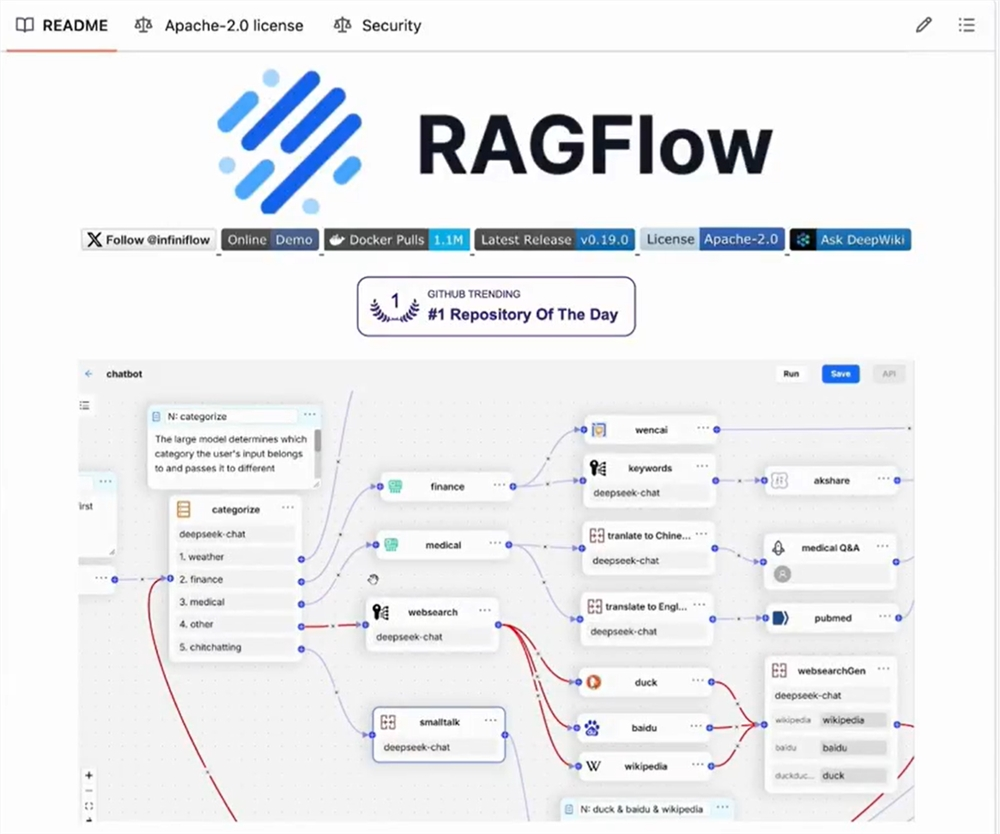
\includegraphics[width=0.8\linewidth,keepaspectratio]{ragflow}
        \end{center}	
    \end{column}
\end{columns}
\end{frame}

%%%%%%%%%%%%%%%%%%%%%%%%%%%%%%%%%%%%%%%%%%%%%%%%%%%%%%%%%%%
\begin{frame}[fragile]\frametitle{xpander}
\begin{columns}
    \begin{column}[T]{0.6\linewidth}
      \begin{itemize}
        \item Framework-agnostic backend for AI agents
        \item Manages memory, tools, events, multi-user state
        \item UI-based agent development with low-code support
        \item Supports testing and deployment of agents
        \item Works with LlamaIndex, CrewAI, and more
        \item Includes guardrails for safe agent behavior
        \item Great for building production-ready agent systems
        \item GitHub: \texttt{github.com/xpander-ai/xpander.ai}
      \end{itemize}
    \end{column}
    \begin{column}[T]{0.4\linewidth}
        \begin{center}
        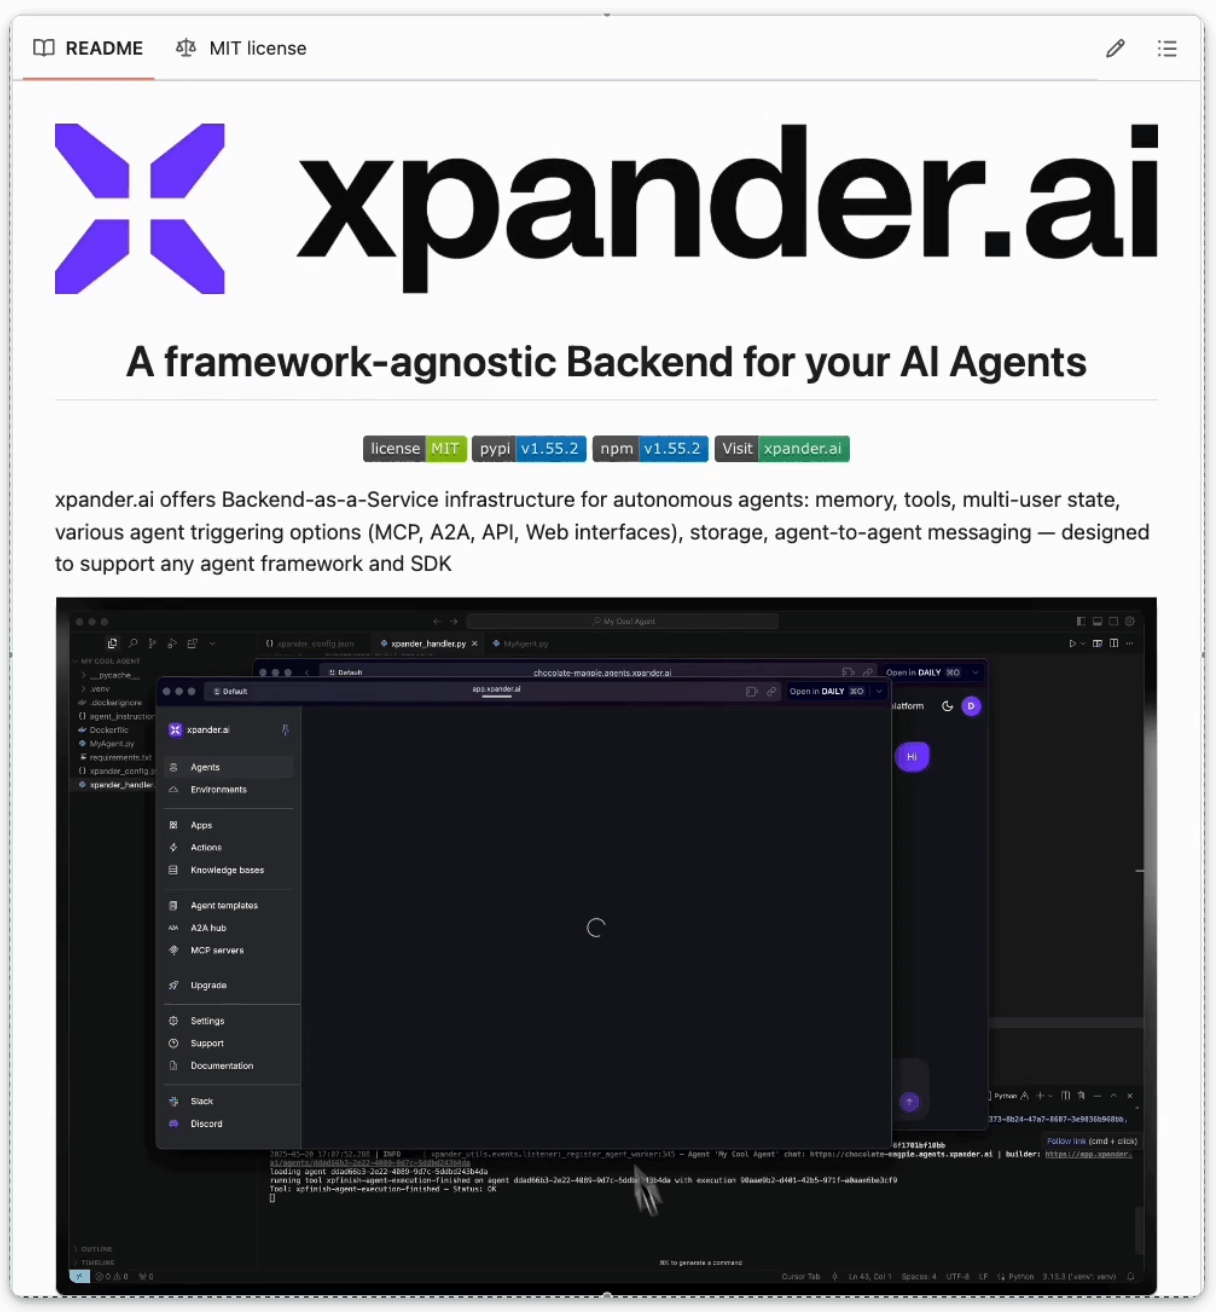
\includegraphics[width=0.8\linewidth,keepaspectratio]{xpander}
        \end{center}	
    \end{column}
\end{columns}
\end{frame}

%%%%%%%%%%%%%%%%%%%%%%%%%%%%%%%%%%%%%%%%%%%%%%%%%%%%%%%%%%%
\begin{frame}[fragile]\frametitle{Transformer Lab}
\begin{columns}
    \begin{column}[T]{0.6\linewidth}
      \begin{itemize}
        \item UI-based app to experiment with LLMs
        \item Train, fine-tune, or chat with models
        \item Drag-n-drop interface for RAG workflows
        \item One-click download of popular LLMs
        \item Includes built-in logging and debugging tools
        \item Fully local and open-source
        \item Supports models like DeepSeek, Gemma, etc.
        \item GitHub: \texttt{github.com/transformerlab/transformerlab-app}
      \end{itemize}
    \end{column}
    \begin{column}[T]{0.4\linewidth}
        \begin{center}
        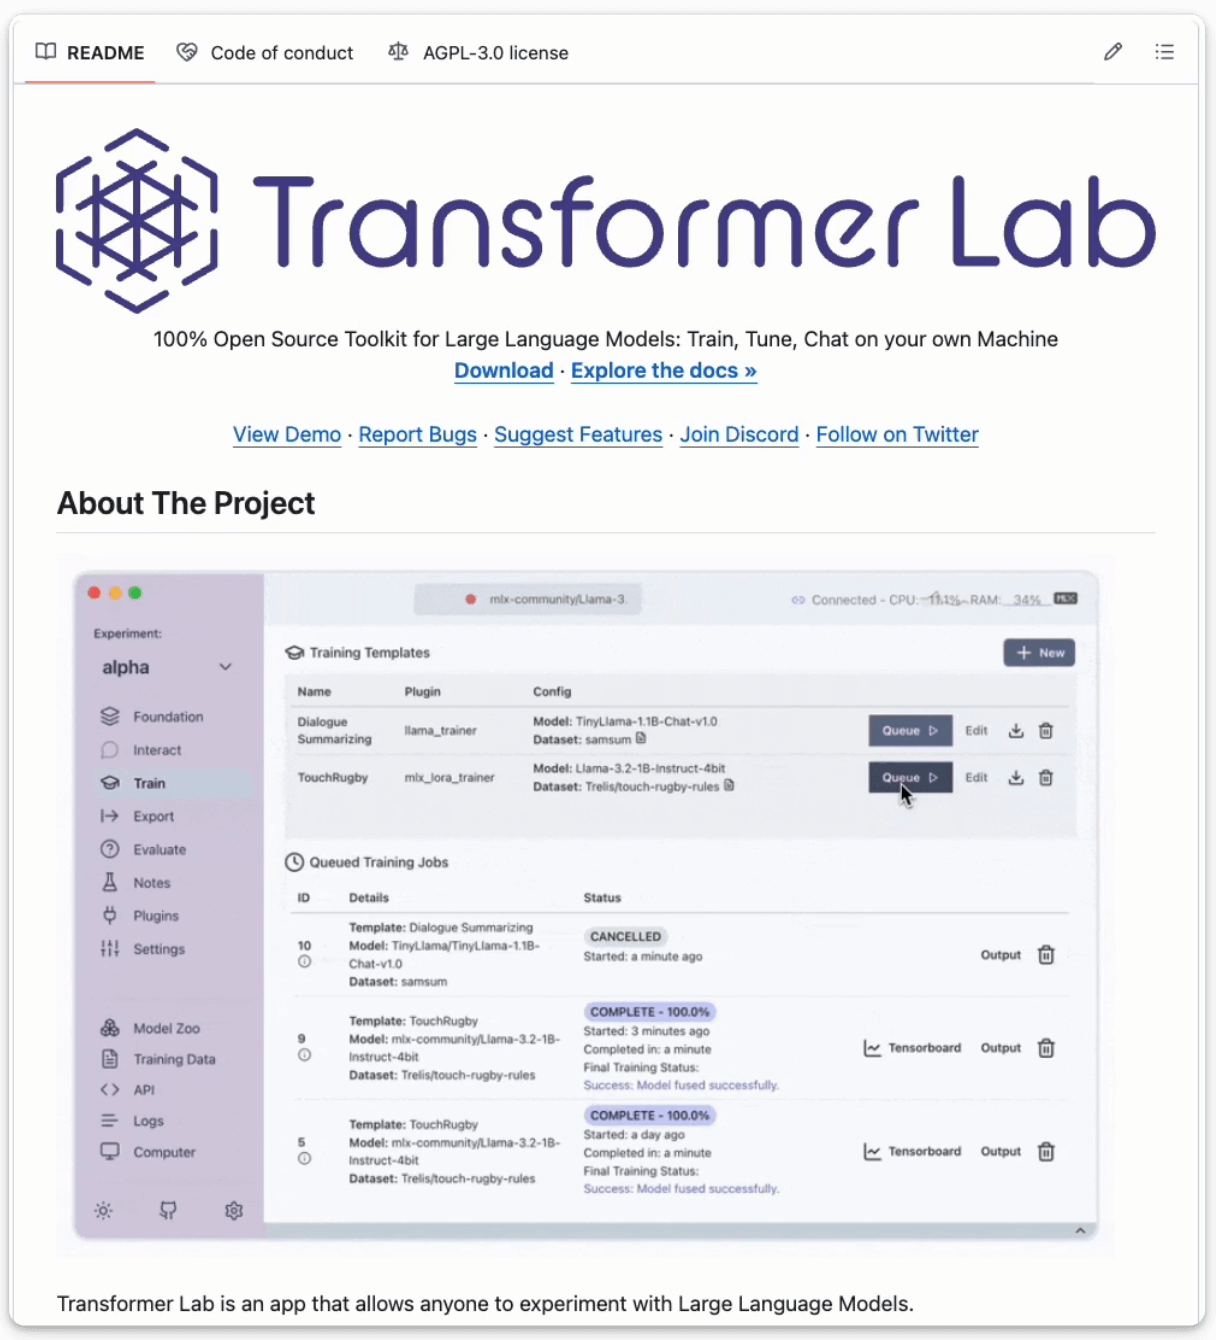
\includegraphics[width=0.8\linewidth,keepaspectratio]{transformerlab}
        \end{center}	
    \end{column}
\end{columns}
\end{frame}

%%%%%%%%%%%%%%%%%%%%%%%%%%%%%%%%%%%%%%%%%%%%%%%%%%%%%%%%%%%
\begin{frame}[fragile]\frametitle{LLaMA-Factory}
\begin{columns}
    \begin{column}[T]{0.6\linewidth}
      \begin{itemize}
        \item No-code training and fine-tuning of LLMs and VLMs
        \item Supports over 100 open-source models
        \item Handles multimodal fine-tuning with ease
        \item Includes PPO, DPO, and experiment tracking
        \item Built for researchers and practitioners
        \item Very popular with 50k+ GitHub stars
        \item Enables fast experimentation without coding
        \item GitHub: \texttt{github.com/hiyouga/LLaMA-Factory}
      \end{itemize}
    \end{column}
    \begin{column}[T]{0.4\linewidth}
        \begin{center}
        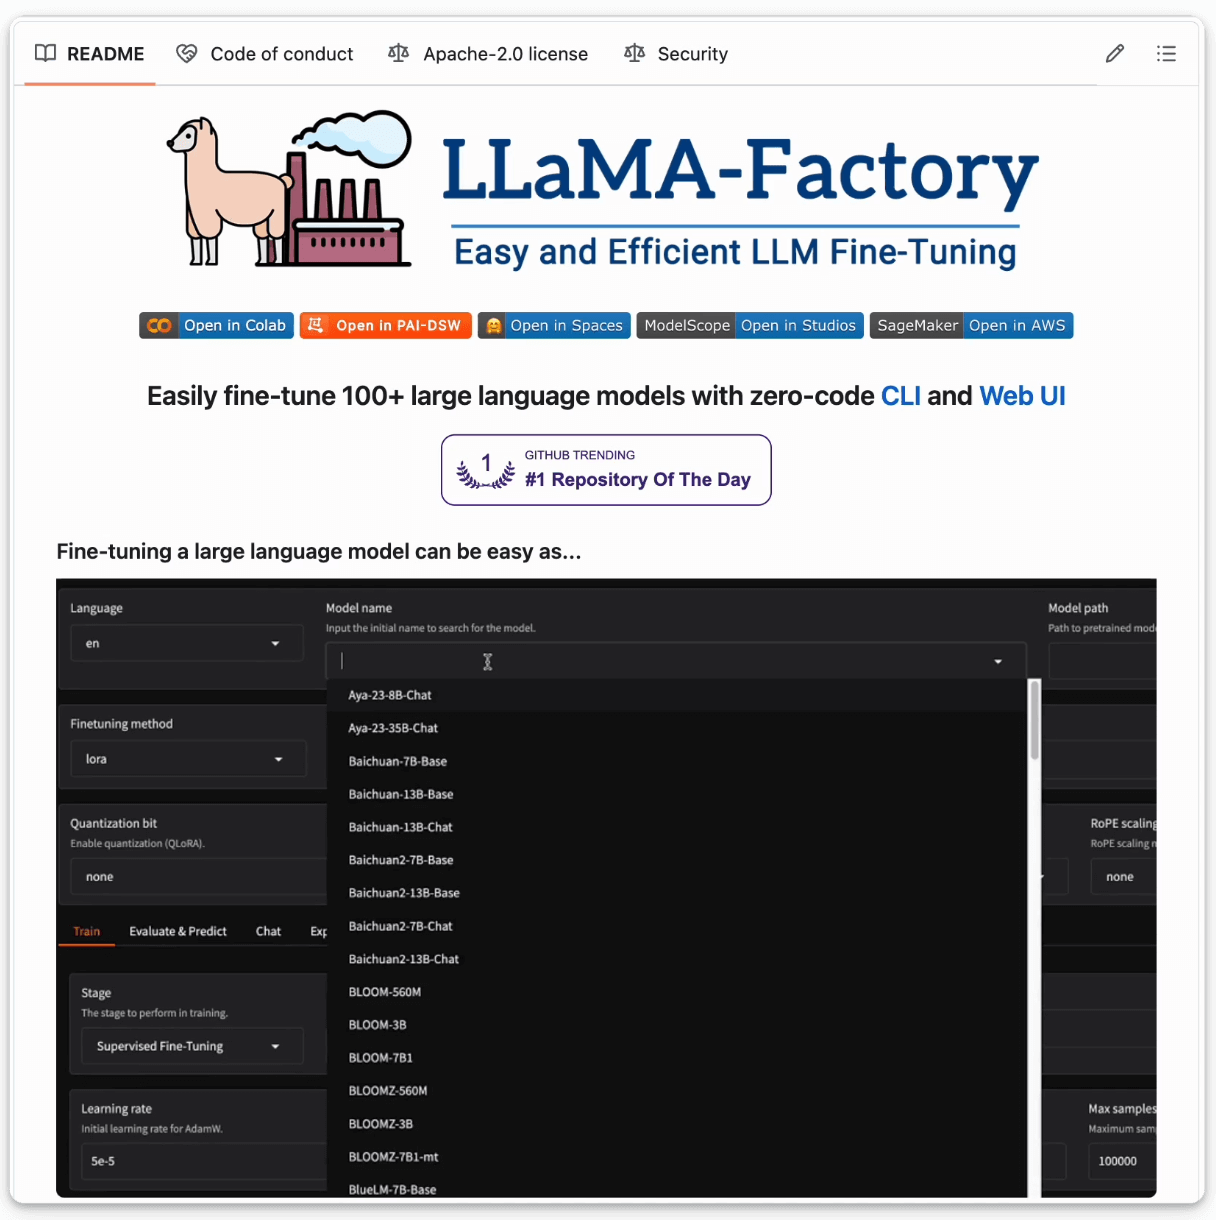
\includegraphics[width=0.8\linewidth,keepaspectratio]{llama-factory}
        \end{center}	
    \end{column}
\end{columns}
\end{frame}

%%%%%%%%%%%%%%%%%%%%%%%%%%%%%%%%%%%%%%%%%%%%%%%%%%%%%%%%%%%
\begin{frame}[fragile]\frametitle{Langflow}
\begin{columns}
    \begin{column}[T]{0.6\linewidth}
      \begin{itemize}
        \item Drag-and-drop interface to build AI agents
        \item Supports all major LLMs and vector databases
        \item Easily build, test, and deploy agent workflows
        \item No-code environment for rapid prototyping
        \item Visualizes agent logic and data flow
        \item Extremely popular: 82k+ GitHub stars
        \item Suitable for beginners and pros alike
        \item GitHub: \texttt{github.com/langflow-ai/langflow}
      \end{itemize}
    \end{column}
    \begin{column}[T]{0.4\linewidth}
        \begin{center}
        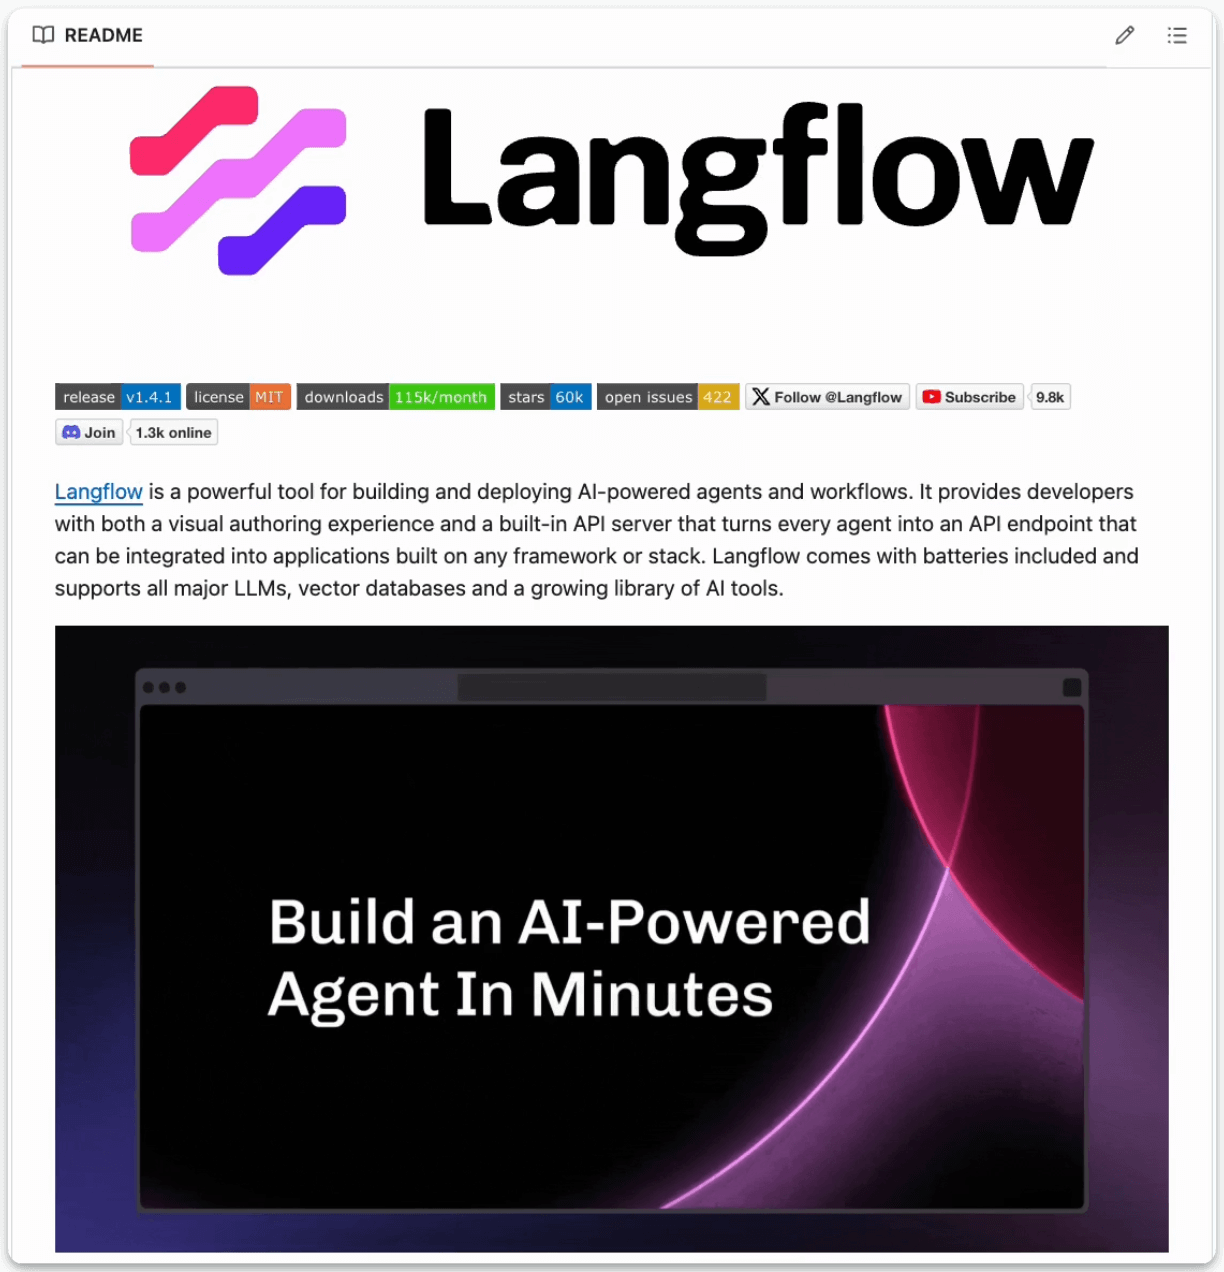
\includegraphics[width=0.8\linewidth,keepaspectratio]{langflow}
        \end{center}	
    \end{column}
\end{columns}
\end{frame}

%%%%%%%%%%%%%%%%%%%%%%%%%%%%%%%%%%%%%%%%%%%%%%%%%%%%%%%%%%%
\begin{frame}[fragile]\frametitle{AutoAgent}
\begin{columns}
    \begin{column}[T]{0.6\linewidth}
      \begin{itemize}
        \item Zero-code agent framework using natural language
        \item Full LLM support out of the box
        \item Built-in self-managing vector DB
        \item Includes ReAct and function-calling modes
        \item Enables quick prototyping and deployment
        \item Ideal for non-technical users
        \item Fully open-source with 5k GitHub stars
        \item GitHub: \texttt{github.com/HKUDS/AutoAgent}
      \end{itemize}
    \end{column}
    \begin{column}[T]{0.4\linewidth}
        \begin{center}
        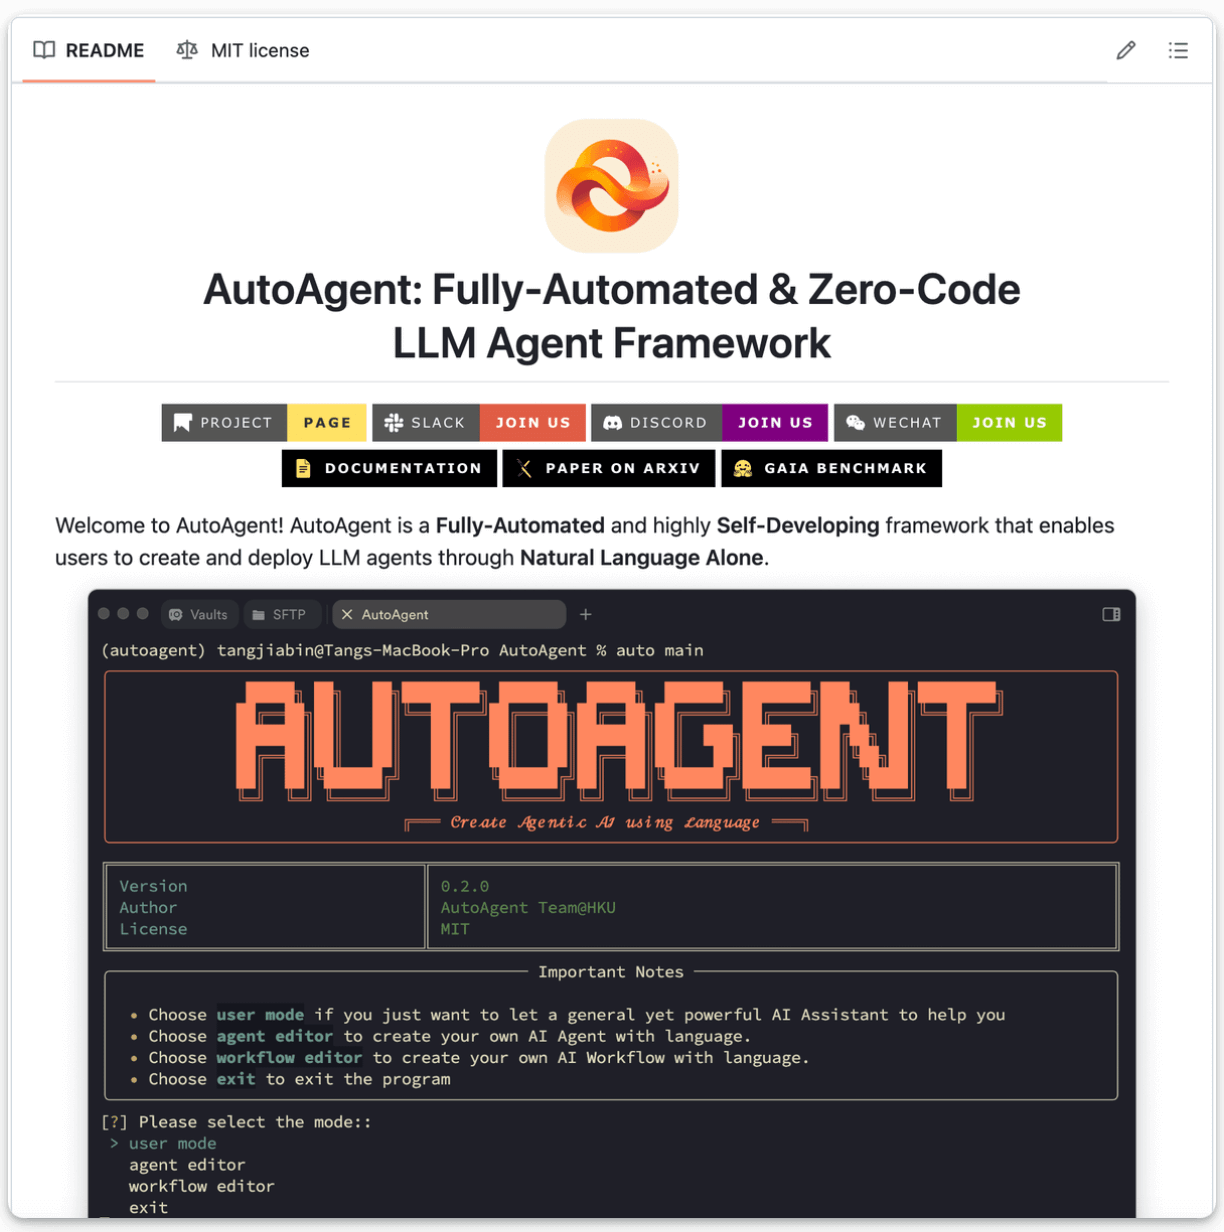
\includegraphics[width=0.8\linewidth,keepaspectratio]{autoagent}
        \end{center}	
    \end{column}
\end{columns}
\end{frame}


%%%%%%%%%%%%%%%%%%%%%%%%%%%%%%%%%%%%%%%%%%%%%%%%%%%%%%%%%%%%%%%%%%%%%%%%%%%%%%%%%%
\begin{frame}[fragile]\frametitle{AI Agents Learning Road-map}
		\begin{center}
		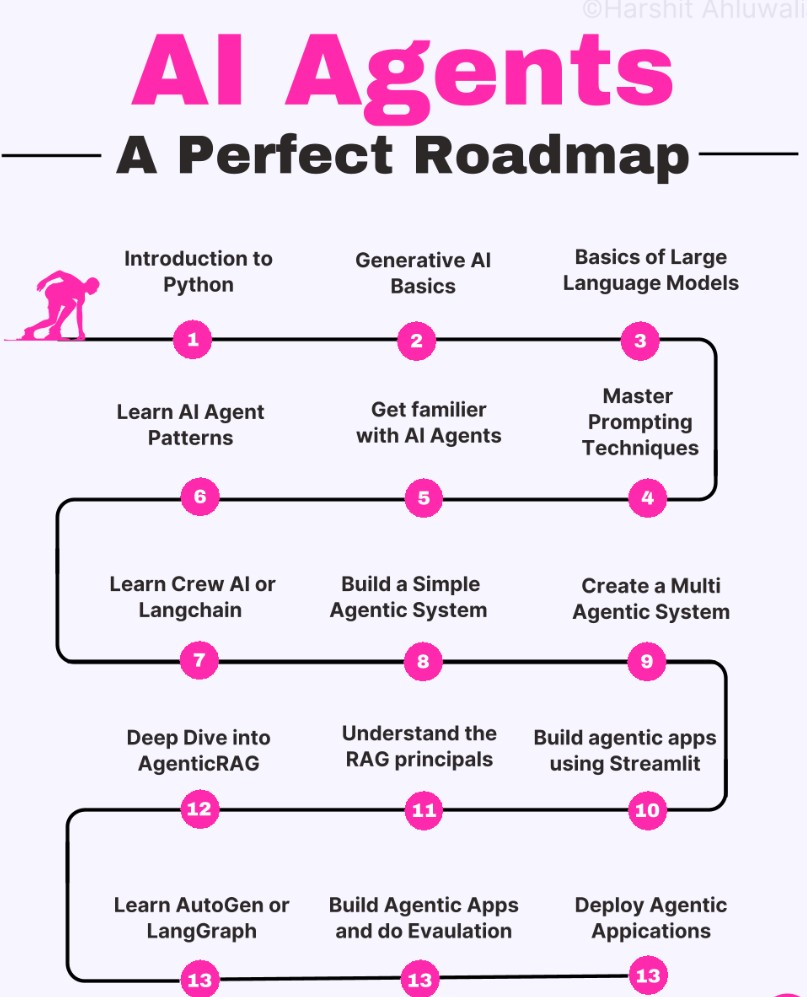
\includegraphics[width=0.5\linewidth,keepaspectratio]{aiagents4}
		
		{\tiny (Ref: LinkedIn post by Harshit Ahluwalia)}
		
		\end{center}
		
\end{frame}